\documentclass[11pt,a4paper]{article}

\usepackage[margin=25mm]{geometry}
\usepackage{booktabs}
\usepackage{graphicx}
\usepackage{float}
\usepackage{hyperref}
\usepackage{siunitx}
\usepackage{xcolor}
\usepackage{longtable}
\usepackage{array}

\graphicspath{{../../results/figures/stage_a_baseline/}}

\title{Stage A Baseline Report\\Adaptive Remeshing Phase-Field Thesis}
\author{Pruthvi Raj Vakkalagadda}
\date{Updated 2026-07-14}

\begin{document}
\maketitle

\section*{Purpose and Maintenance Rule}

This report is the single living \LaTeX{} report for Stage A: environment/toolchain verification, original Molnar source preservation, unchanged one-element verification, and unchanged notched-benchmark reproduction. It should be updated after each Stage A gate until a new report file is intentionally opened for the next thesis stage. It is a reproducibility and scientific-review report, not a claim that remeshing or state transfer has been validated.

\section*{Current Gate Status}

\begin{table}[H]
\centering
\caption{Project gate status at this report revision.}
\begin{tabular}{@{}ll@{}}
\toprule
Gate & Status \\
\midrule
WP0 environment/toolchain gate & Passed locally \\
WP1 one-element technical gate & Passed \\
WP1 one-element scientific gate & Passed provisionally \\
WP2 single-notch technical gate & Passed \\
WP2 single-notch scientific comparison & Pending \\
MISESERI pre-refinement & Blocked until WP2 review \\
Remeshing/state transfer & Not started \\
\bottomrule
\end{tabular}
\end{table}

\section{WP0 Environment and Toolchain}

The local environment inspection recorded Abaqus 2024, Abaqus Python 3.10.5, Windows 11, 12 logical processors, approximately \SI{23.35}{GiB} physical memory, GNU Fortran availability, and the absence of a usable Intel Fortran toolchain on a plain shell path. The successful user-subroutine smoke gate then established the required clean-shell sequence: load Visual Studio 2022 Build Tools with \texttt{vcvars64.bat}, then Intel oneAPI with \texttt{setvars.bat intel64}. In that environment, Abaqus used Intel \texttt{ifx} 2026.0.0 for compilation and Microsoft \texttt{LINK} 14.44.35226.0 for linking.

This is a local observed toolchain pass only. It is not an official Abaqus 2024--oneAPI 2026 support claim and it does not validate any phase-field formulation.

\section{Preserved Molnar Baseline}

The Molnar and Gravouil 2017 supplementary package is preserved under \texttt{models/baseline\_original/molnar\_gravouil\_2017/}. The unchanged run copies are made from that baseline and hash-checked before execution.

\begin{table}[H]
\centering
\caption{Preserved source/deck checksums used in completed gates.}
\begin{tabular}{@{}lll@{}}
\toprule
Gate & File & SHA-256 \\
\midrule
One element & \texttt{OneElement.for} & \texttt{8688a21a987a0348f4211cb90e365a60902dce922294a915a48644c8dae067e2} \\
One element & \texttt{OneElement.inp} & \texttt{9b63615bbe335872de197b96ca0253769f4a237c1e2e384294a1d204c462f220} \\
Single notch & \texttt{SingleNotch.for} & \texttt{18944e5bb2a3b7973fd0d4bff03f8e078eef667965343d8a29156d093f53f5f1} \\
Single notch & \texttt{SingleNotch.inp} & \texttt{89ce3f32e396b0e484be6753a272dd6bbb2a2f9daff426d6a57419f57d665b72} \\
\bottomrule
\end{tabular}
\end{table}

\section{WP1 One-Element Verification}

The unchanged one-element example passed the technical gate and the source-defined scientific check under provisional numerical tolerances. The validator opens the unchanged ODB read-only, checks all \texttt{SDV1}--\texttt{SDV16}, processes every frame and integration point, and writes CSV, JSON, and Markdown evidence.

The one-element verification established:
\begin{itemize}
  \item plane-strain undamaged elasticity;
  \item degraded stress using the phase field applied by the displacement element;
  \item homogeneous phase-field relation;
  \item monotonic history field;
  \item no phase-field healing during unloading;
  \item consistency across the four integration points.
\end{itemize}

The maximum phase-relation absolute error was approximately \(5.98\times10^{-7}\). The undamaged-stress absolute errors remained below \(1.90\times10^{-6}\). The largest \texttt{SDV14}-\texttt{SDV15} difference was approximately \(4.88\times10^{-3}\), interpreted as a staggered-update difference between the phase field used by the displacement solve and the phase-element value, not as automatic source corruption.

\section{WP2 Unchanged Single-Notch Technical Benchmark}

The unchanged Molnar single-notch tension benchmark ran from
\texttt{runs/molnar\_single\_notch\_unchanged/20260714\_technical\_gate\_local/}. The run classification is \texttt{technical\_pass\_scientific\_unchecked}.

\begin{table}[H]
\centering
\caption{Single-notch technical gate checks.}
\begin{tabular}{@{}ll@{}}
\toprule
Check & Status \\
\midrule
Original source/deck preserved and hash-matched & Pass \\
Compile and link & Pass \\
Input processing & Pass \\
Abaqus/Standard completion & Pass \\
\texttt{.sta} completion status & Pass \\
ODB readability & Pass \\
Automated RF--U/SDV extraction & Pass \\
Reference RF--U comparison & Pending \\
Crack-path comparison & Pending \\
Energy-response validation & Pending \\
\bottomrule
\end{tabular}
\end{table}

The model contains 3,998 nodes and 11,790 layered elements. The extraction produced 72 RF--U/phase states. Field outputs in both steps include \texttt{RF}, \texttt{U}, and \texttt{SDV1}--\texttt{SDV16}. The ODB is about \SI{88}{MB} and is kept local rather than mirrored into Git or handoff.

\begin{figure}[H]
\centering
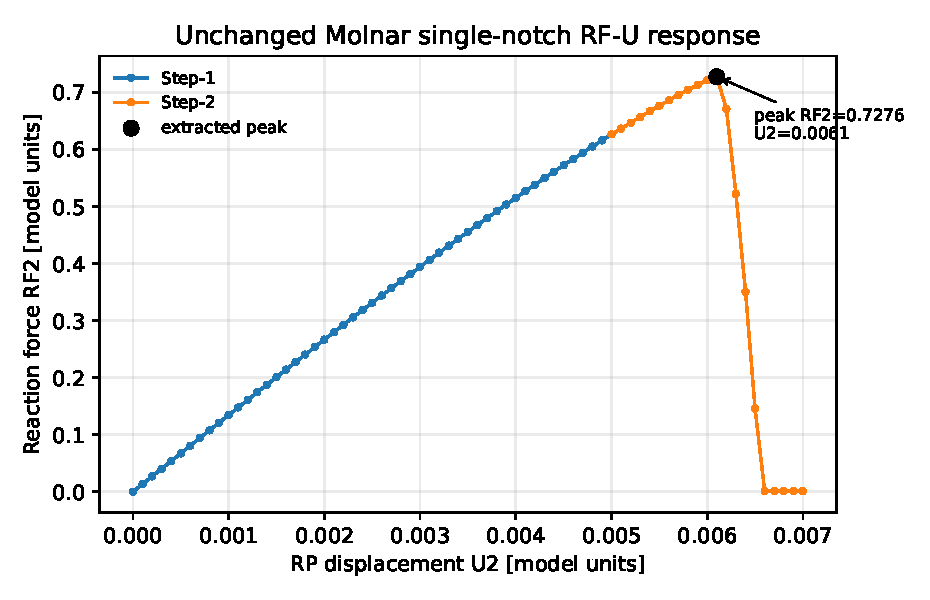
\includegraphics[width=0.85\linewidth]{single_notch_rf_u_curve.pdf}
\caption{Extracted reaction force versus applied displacement for the unchanged Molnar single-notch benchmark. The curve is not yet compared to the Molnar reference curve.}
\end{figure}

\begin{figure}[H]
\centering
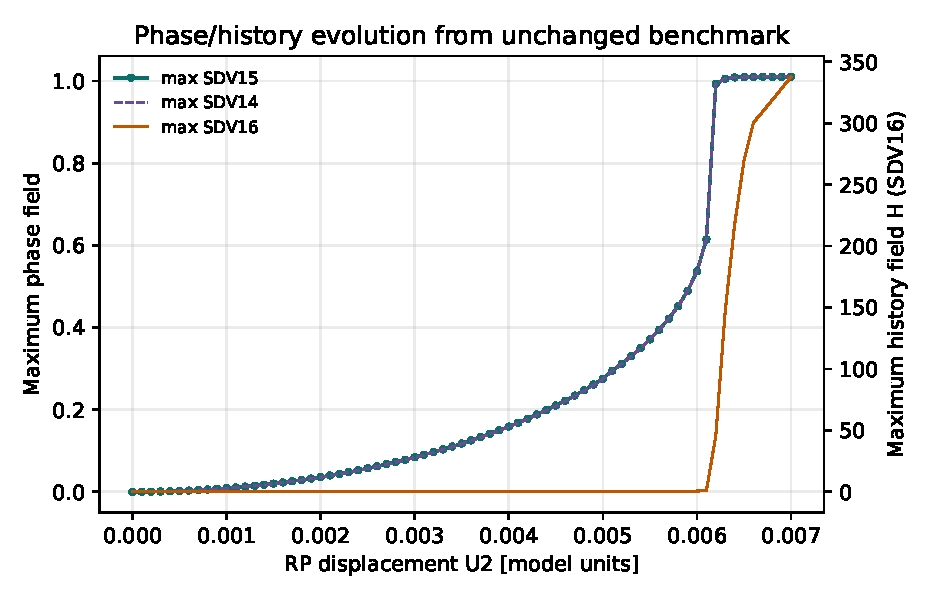
\includegraphics[width=0.85\linewidth]{single_notch_phase_history_vs_u.pdf}
\caption{Maximum \texttt{SDV14}, \texttt{SDV15}, and \texttt{SDV16} versus applied displacement. \texttt{SDV16} is the local history field \(H\), not global fracture energy.}
\end{figure}

\begin{table}[H]
\centering
\caption{Matched displacement states extracted from the unchanged benchmark.}
\begin{tabular}{@{}rrrr@{}}
\toprule
\(U_2\) & \(RF_2\) & \(\max(\mathrm{SDV15})\) & \(\max(\mathrm{SDV16})\) \\
\midrule
0.002 & 0.266812 & 0.03598 & 0.02080 \\
0.005 & 0.626645 & 0.27554 & 0.21283 \\
0.006 & 0.721406 & 0.53678 & 0.64532 \\
0.007 & 0.001395 & 1.01049 & 337.78018 \\
\bottomrule
\end{tabular}
\end{table}

The matched states show increasing damage followed by near-complete loss of load-carrying capacity. This qualitative sequence is compatible with failure, but the shape, peak, post-peak drop, and crack evolution still require quantitative comparison with Molnar and Gravouil's reference behavior before any scientific pass is claimed.

\section{Phase Contours and Bound Diagnostic}

Figures~\ref{fig:phase-raw} and~\ref{fig:phase-clipped} show the raw and display-clipped \texttt{SDV15} contours at the matched displacement states. The clipped plots are for visualization only. Quantitative calculations must use raw values.

\begin{figure}[H]
\centering
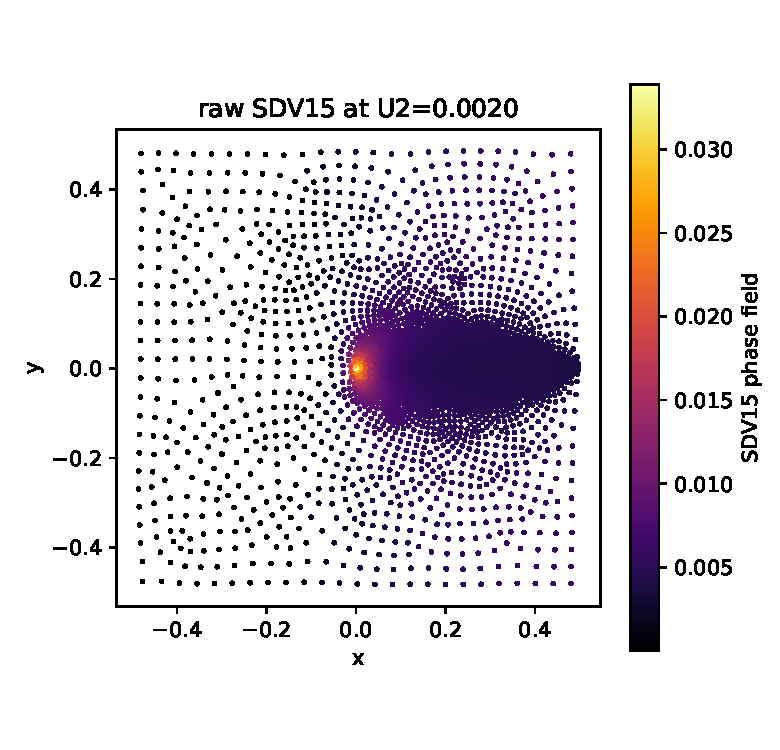
\includegraphics[width=0.48\linewidth]{matched_state_01_Step-1_frame_0020_raw_sdv15.pdf}
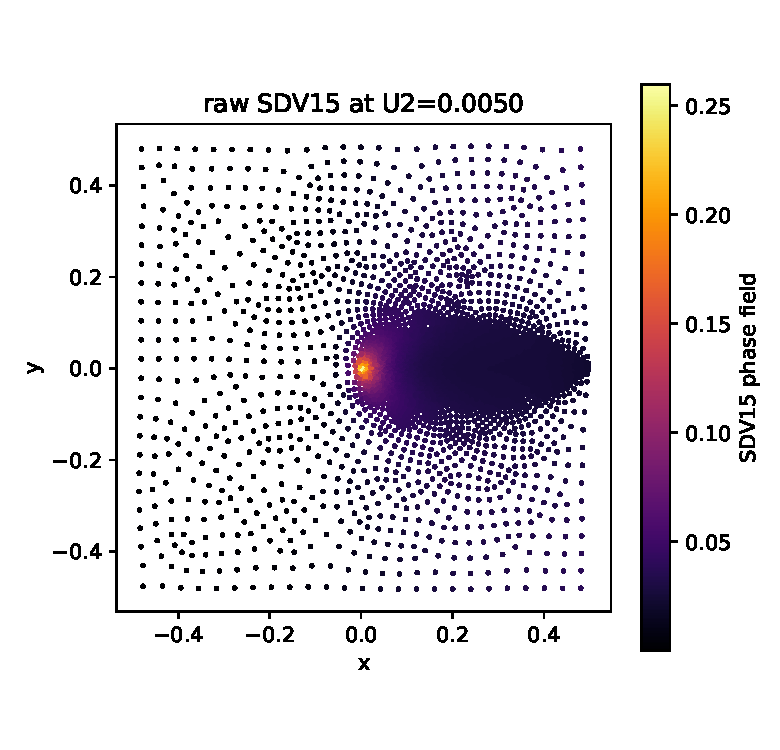
\includegraphics[width=0.48\linewidth]{matched_state_02_Step-1_frame_0050_raw_sdv15.pdf}\\
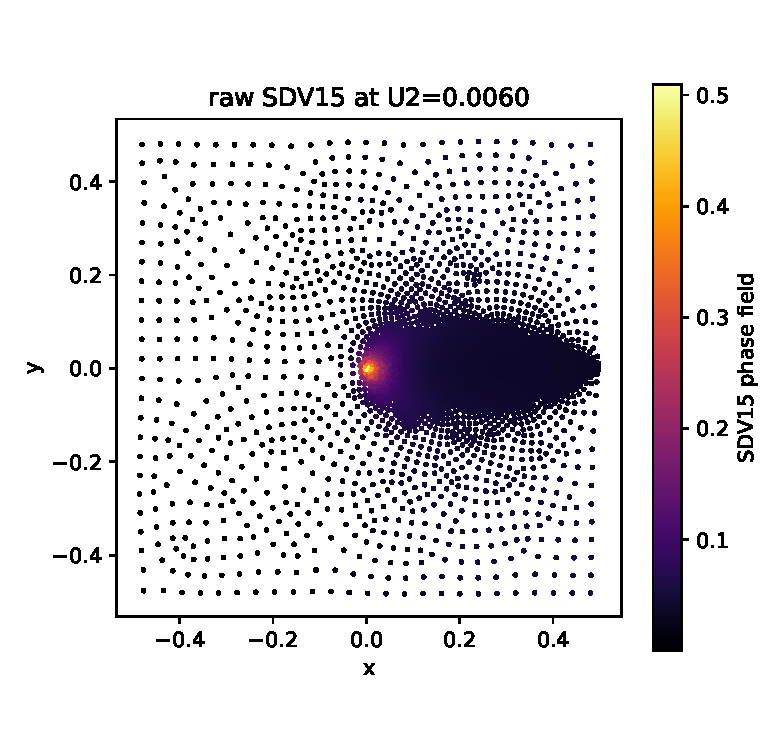
\includegraphics[width=0.48\linewidth]{matched_state_03_Step-2_frame_0010_raw_sdv15.pdf}
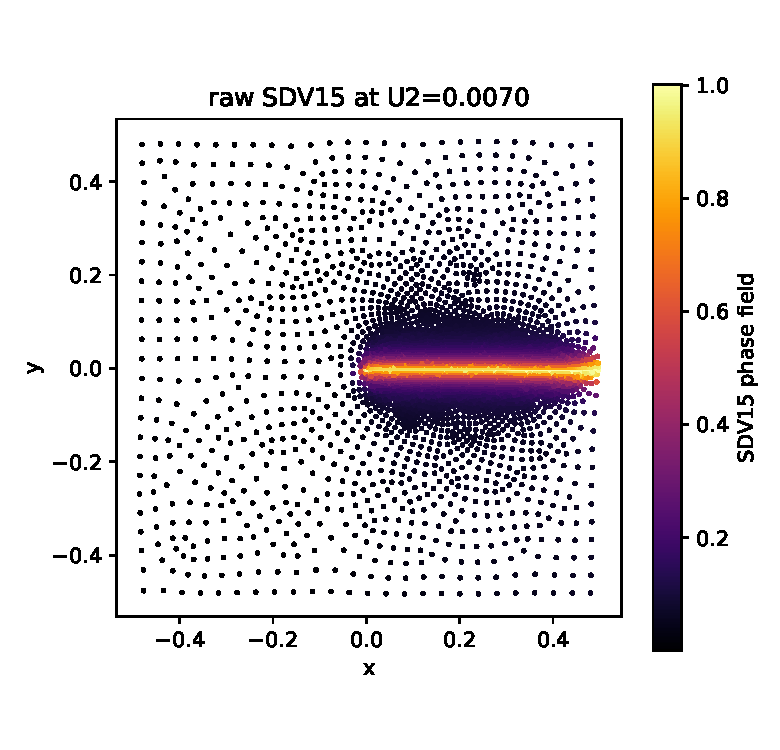
\includegraphics[width=0.48\linewidth]{matched_state_04_Step-2_frame_0020_raw_sdv15.pdf}
\caption{Raw \texttt{SDV15} phase-field contours at \(U_2=0.002,0.005,0.006,0.007\).}
\label{fig:phase-raw}
\end{figure}

\begin{figure}[H]
\centering
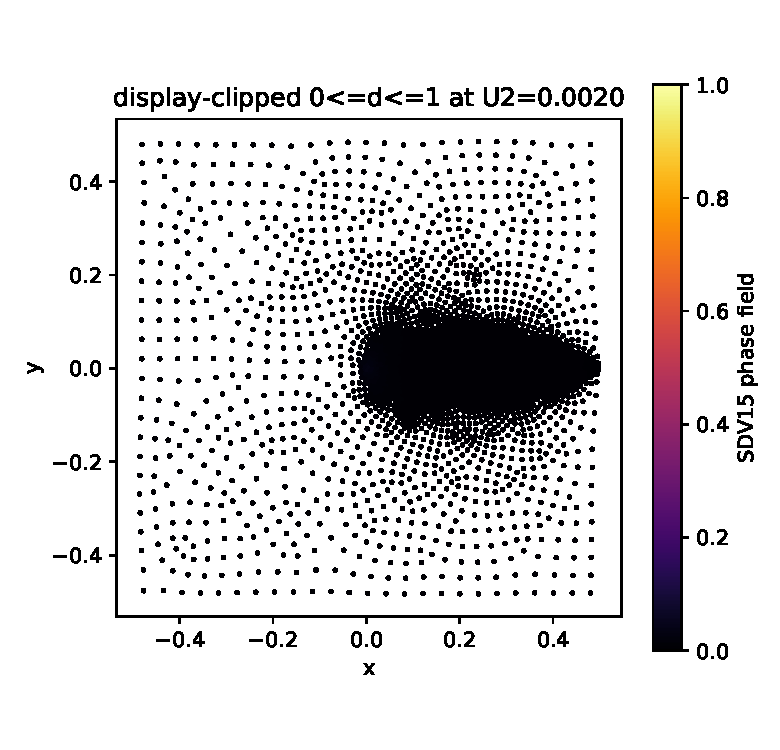
\includegraphics[width=0.48\linewidth]{matched_state_01_Step-1_frame_0020_clipped_sdv15.pdf}
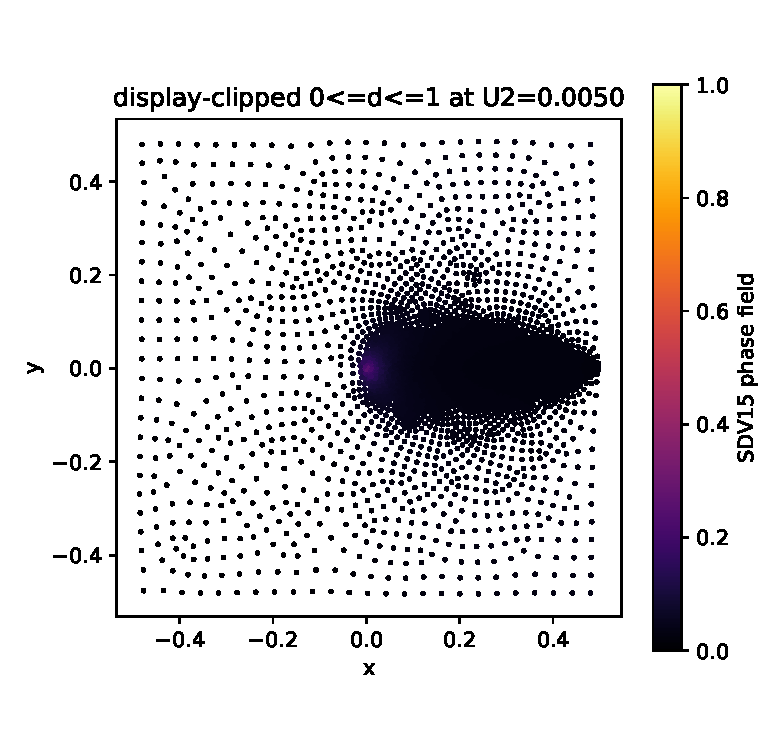
\includegraphics[width=0.48\linewidth]{matched_state_02_Step-1_frame_0050_clipped_sdv15.pdf}\\
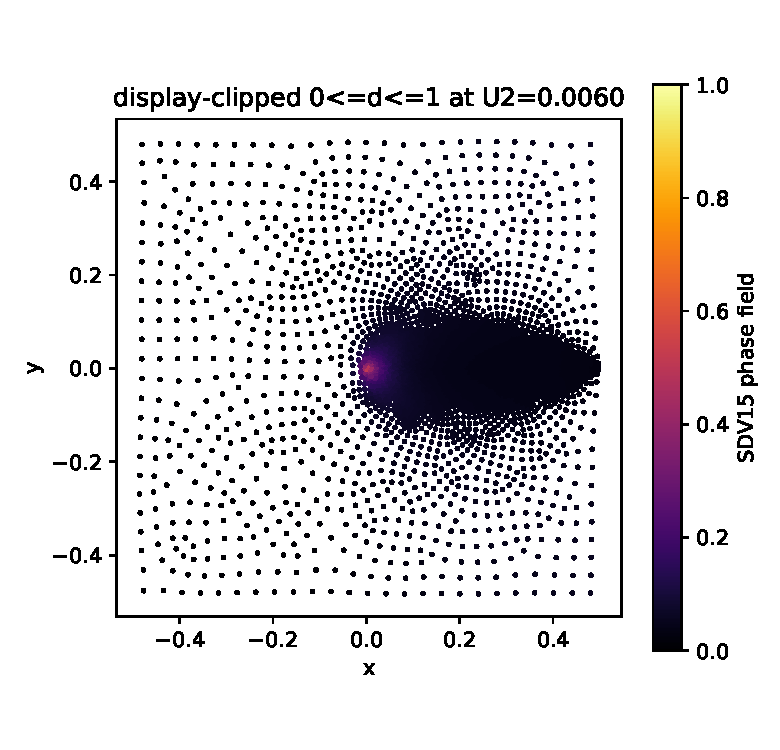
\includegraphics[width=0.48\linewidth]{matched_state_03_Step-2_frame_0010_clipped_sdv15.pdf}
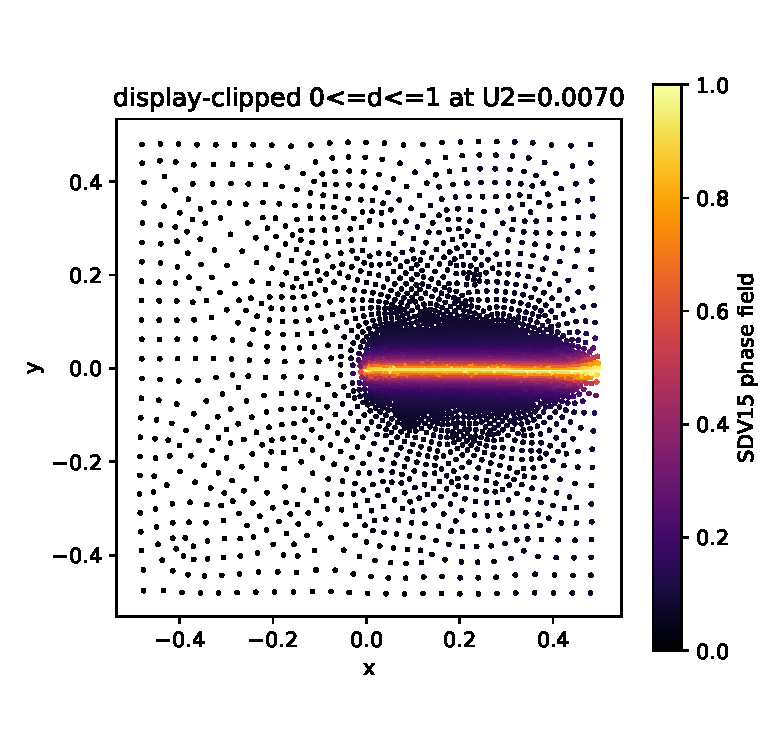
\includegraphics[width=0.48\linewidth]{matched_state_04_Step-2_frame_0020_clipped_sdv15.pdf}
\caption{Display-only \texttt{SDV15} contours clipped to \(0\le d\le1\). These images are for interpretation and must not replace raw values in calculations.}
\label{fig:phase-clipped}
\end{figure}

The final raw value \(\max(\mathrm{SDV15})=1.010493\) is approximately 1.05\% above the nominal phase-field upper bound. The original element calculation does not include an explicit clipping operation, so a small discrete overshoot is possible. This does not invalidate the technical gate, but it is now a required scientific diagnostic:
\begin{itemize}
  \item preserve the raw value;
  \item determine its element, integration point, and first occurrence;
  \item report both raw and display-only clipped contours;
  \item check whether \texttt{SDV14}, \texttt{SDV15}, or both overshoot;
  \item verify whether overshoot is limited to the final unstable propagation stage;
  \item do not silently clip values in quantitative calculations.
\end{itemize}

\section{Pending Scientific Comparison}

The next validator should compare the unchanged result against the appropriate curve in Molnar and Gravouil's Fig.~7 and the tensile crack pattern in Fig.~6. The report should then add:
\begin{itemize}
  \item initial stiffness;
  \item peak reaction force and displacement at peak;
  \item force at matched displacement values;
  \item normalized RF--U curve error;
  \item post-peak drop and residual force;
  \item crack initiation location and straight Mode-I propagation from the notch;
  \item thresholded crack path using a declared \(d\)-threshold;
  \item crack-line deviation from the expected horizontal ligament;
  \item monotonic \texttt{SDV16} and persistent-point non-decreasing \texttt{SDV15};
  \item count and magnitude of values below zero or above one;
  \item \texttt{SDV14}/\texttt{SDV15} staggered difference.
\end{itemize}

Energy terminology must remain precise. \texttt{SDV16} is the local history field \(H\), not global fracture energy. Its maximum value of 337.78 must not be labelled fracture energy. The source identifies \texttt{SDV12} as degraded strain energy density, \texttt{SDV13} as undamaged elastic energy density, and \texttt{SDV16} as the history field. Any global energy comparison requires a properly integrated energy measure.

\section*{Reproducibility Files}

\begin{itemize}
  \item One-element scientific validator: \texttt{scripts/validation/check\_molnar\_one\_element.py}
  \item Single-notch extractor: \texttt{scripts/postprocessing/extract\_molnar\_single\_notch.py}
  \item Report figure generator: \texttt{scripts/postprocessing/generate\_stage\_a\_report\_figures.py}
  \item One-element evidence: \texttt{runs/molnar\_one\_element\_unchanged/20260714\_technical\_gate\_local/scientific\_check/}
  \item Single-notch evidence: \texttt{runs/molnar\_single\_notch\_unchanged/20260714\_technical\_gate\_local/}
  \item Report figures: \texttt{results/figures/stage\_a\_baseline/}
  \item Report tables: \texttt{results/tables/stage\_a\_baseline/}
\end{itemize}

\end{document}
